% This LaTeX document needs to be compiled with XeLaTeX.
\documentclass[10pt]{article}
\usepackage[utf8]{inputenc}
\usepackage{ucharclasses}
\usepackage{graphicx}
\usepackage[export]{adjustbox}
\graphicspath{ {./images/} }
\usepackage{hyperref}
\hypersetup{colorlinks=true, linkcolor=blue, filecolor=magenta, urlcolor=cyan,}
\urlstyle{same}
\usepackage{amsmath}
\usepackage{amsfonts}
\usepackage{amssymb}
\usepackage[version=4]{mhchem}
\usepackage{stmaryrd}
\usepackage{polyglossia}
\usepackage{fontspec}
\setmainlanguage{spanish}
\setotherlanguages{portuguese, thai}
\newfontfamily\thaifont{Noto Serif Thai}
\newfontfamily\lgcfont{CMU Serif}
\setDefaultTransitions{\lgcfont}{}
\setTransitionsFor{Thai}{\thaifont}{\lgcfont}

\title{Victor Ribeiro Carreira }

\author{}
\date{}


%New command to display footnote whose markers will always be hidden
\let\svthefootnote\thefootnote
\newcommand\blfootnotetext[1]{%
  \let\thefootnote\relax\footnote{#1}%
  \addtocounter{footnote}{-1}%
  \let\thefootnote\svthefootnote%
}

%Overriding the \footnotetext command to hide the marker if its value is `0`
\let\svfootnotetext\footnotetext
\renewcommand\footnotetext[2][?]{%
  \if\relax#1\relax%
    \ifnum\value{footnote}=0\blfootnotetext{#2}\else\svfootnotetext{#2}\fi%
  \else%
    \if?#1\ifnum\value{footnote}=0\blfootnotetext{#2}\else\svfootnotetext{#2}\fi%
    \else\svfootnotetext[#1]{#2}\fi%
  \fi
}

\begin{document}
\maketitle
\begin{center}
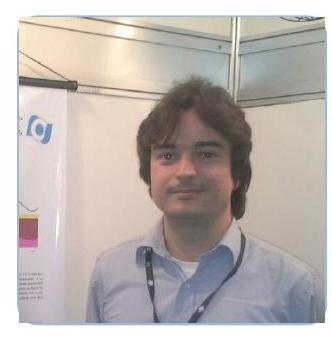
\includegraphics[max width=\textwidth]{2024_06_29_acf33ffb82555b8284bcg-01}
\end{center}

Endereço para acessar este CV: \href{http://lattes.cnpq.br/9663791782095105}{http://lattes.cnpq.br/9663791782095105} ID Lattes: 9663791782095105

Última atualização do currículo em 03/10/2022

Atualmente trabalha como pesquisador de pós-doutorado na Universidade Federal Fluminense integrando a equipe do projeto Ressurgência. Possui doutorado em Geofísica pelo Observatório Nacional, na área de geofísica aplicada à Geofísica de Exploração com ênfase em meta-heurística e métodos de inteligência artificial aplicados à dados de perfilagem geofísica, em Bacias Sedimentares (2021).Mestrado em Geofísica pelo Observatório Nacional na área de Métodos Potencias e Eletromagnéticos (2015), e graduação em Geologia pela Universidade Federal do Rio de Janeiro (2012). Em sua graduação, trabalhou como estagiário (bolsista COPPETEC), no projeto "Aplicação da Bioestratigrafia da Radiolários ao Refinamento Estratigráfico do Cretáceo e Paleógeno nas Bacias Brasileiras", financiado pelo BPA/Cenpes/Petrobras/ e vinculado ao LAFO - UFRJ. Em seu mestrado, desenvolveu estudos relativos ao embasamento da Bacia do Paraná e a Bacia Sedimentar correlata através do uso de Métodos Potenciais e Magnetotelúrico. Em seu doutorado, desenvolveu uma nova metodologia aplicadas à área de Inteligência Artificial para reconhecimento de padrões litológicos e um novo modelo gerador de pseudo-poços baseados em seções geológicas e sísmica 2D. (Texto informado pelo autor)

\section*{Identificação}
\section*{Nome}
\section*{Victor Ribeiro Carreira}
Nome em citações

bibliográficas

CARREIRA, V. R.;CARREIRA, VICTOR

\section*{Lattes iD}
\section*{(๑)}
\href{http://lattes.cnpq.br/9663791782095105}{http://lattes.cnpq.br/9663791782095105}

\section*{Orcid iD}
? (D) \href{https://orcid.org/0000-0002-22888739}{https://orcid.org/0000-0002-22888739}

\section*{Endereço}
\section*{Endereço \\
 Profissional}
Ministério da Educação, Universidade

Federal Fluminense.

Rua Mário Santos Braga

Centro

24020140 - Niterói, RJ - Brasil

Telefone: (21) 26292428

Ramal: 513

URL da Homepage: \href{https://www.uff.br/}{https://www.uff.br/}

Doutorado em Geofísica.

Observatório Nacional, ON, Brasil.

Título: Inteligência Artificial aplicada ao reconhecimento de padrões litológicos, Ano de obtenção: 2021.

Orientador: (9) Cosme Ferreira da Ponte Neto.

Coorientador: Rodrigo Bijani Santos.

Bolsista do(a): Fundação Carlos Chagas Filho de Amparo à Pesquisa do Estado do RJ, FAPERJ, Brasil.

\section*{2013 - 2015}
Mestrado em Geofísica.

Observatório Nacional, ON, Brasil.

Título: Contribuição para o entendimento das estruturas geológicas da Bacia do Paraná utilizando métodos potenciais., Ano de Obtenção: 2015.

Orientador: Emanuele Francesco La Terra

Coorientador: Sergio Luiz Fontes.

Bolsista do(a): Conselho Nacional de Desenvolvimento Científico e Tecnológico, CNPq, Brasil

Palavras-chave: Métodos Potenciais. Grande área: Ciências Exatas e da Terra Setores de atividade: Atividades de Apoio à Extração de Minerais.

2007 - 2012

Graduação em Geologia.

Universidade Federal do Rio de Janeiro, UFRJ, Brasil.

Título: O GÁS DE FOLHELHO: UMA NOVA FRONTEIRA.

Orientador: José Mário Coelho.

Bolsista do(a): Fundação coordenação de projetos, pesquisa e estudos tecnológicos, COPPETEC, Brasil.

2002 - 2004

Curso técnico/profissionalizante.

Centro Federal de Educação Tecnológica de Química, CEFETEQ, Brasil.

Pós-doutorado

Pós-Doutorado.

Universidade Federal Fluminense, UFF, Brasil.

Bolsista do(a): Fundação Euclides da Cunha, FEC, Brasil.

Grande área: Ciências Exatas e da Terra

Grande Área: Ciências Exatas e da Terra / Área: Geociências / Subárea: Inteligência

Artificial.

Grande Área: Ciências Exatas e da Terra /

Área: Geociências / Subárea:

Modelagem.

Formação Complementar

2013 - 2013

Mapeamento e processamento com o geosoftware. (Carga horária: $30 \mathrm{~h}$ ).

Observatório Nacional, ON, Brasil.

\section*{Atuação Profissional}
\section*{Universidade Federal Fluminense, UFF, Brasil.}
Vínculo institucional

\section*{2022 - Atual}
Vínculo: Bolsista, Enquadramento Funcional: Pesquisador de pósdoutorado, Carga horária: 40

Vínculo institucional

\section*{2021 - 2022}
\begin{center}
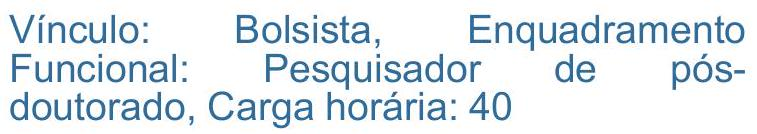
\includegraphics[max width=\textwidth]{2024_06_29_acf33ffb82555b8284bcg-03}
\end{center}

Atividades

\section*{12/2021 - Atual}
Pesquisa e desenvolvimento, Departamento de Geoquímica.

Linhas de pesquisa

Modelagem

Observatório Nacional, ON, Brasil.

Vínculo institucional

Vínculo: Bolsista, Enquadramento

Funcional: Aluno de pós-graduação\\
(doutorado), Carga horária: 40, Regime: Dedicação exclusiva.

Vínculo institucional

2013 - 2015

Vínculo: Bolsista, Enquadramento Funcional: Aluno de pós-graduação (mestrado), Carga horária: 40, Regime: Dedicação exclusiva.

Vínculo institucional

2013 - 2015

Vínculo: Bolsista, Enquadramento

Funcional: Técnico de campo, Carga horária: 20

Atividades

03/2020 - 04/2021

Ensino, Geofísica, Nível: Graduação

Disciplinas ministradas

Orientação de trabalho final de curso. O método K-Means na classificação de litofácies a partir de perfis geofísicos sintéticos inspirados no campo de Namorado, Bacia de Campos.

03/2018 - 03/2021

Extensão universitária, Observatório Nacional.

Atividade de extensão realizada Capítulo Estudantil SEG e EAGE.

$03 / 2018$ - 03/2020

Direção e administração, Observatório Nacional.

Cargo ou função

Representande Discente.

Extensão universitária, Observatório Nacional

1.

\section*{Modelagem}
Projetos de pesquisa

\section*{2022 - Atual}
Projeto Ressurgência Fase 4 Aperfeiçoamento do programa de modelagem de rocha geradora

Descrição: A presente proposta visa aprimorar e desenvolver novos métodos para a modelagem de fácies orgânica em ambientes marinhos e lacustres, melhorando assim a avaliação do potencial das rochas geradoras. No que concerne a modelagem de fácies orgânica marinha, esta será aprimorada através da automatização dos cálculos de parâmetros-chave do processo de simulação (inserção de calculadoras automatizadas), como por exemplo taxa de sedimentação, paleoprodutividade e fator de preservação de carbono orgânico. Esse aperfeiçoamento tem como foco central maximizar a qualidade dos dados de entrada, visando a obtenção de simulações mais acuradas. Além disso, um segundo foco será a elaboração de um software para a modelagem de fácies orgânica lacustre, para o qual será criada uma nova sequência de etapas lógicas para estimar a qualidade e quantidade do carbono orgânico nesses ambientes. Sendo assim, o desenvolvimento completo, desde a criação do modelo conceitual dos processos-chave até sua completa implementação através de um software será executado neste projeto..

Situação: Em andamento; Natureza: Pesquisa.

Alunos envolvidos: Graduação: (2) I Especialização: (0) / Mestrado acadêmico: (2) / Mestrado profissional: (0) / Doutorado: (2) .

Integrantes: Victor Ribeiro Carreira Coordenador / Ana Luiza Spadano Albuquerque - Integrante / Igor Martins Venancio Padilha de Oliveira - Integrante / Thiago Pereira dos Santos - Integrante I Andre Luiz Belem - Integrante / Emmanoel Vieira da Silva Filho Integrante / Marcelo Corrêa Bernardes -

Integrante / Rut Amelia Díaz Ramos

Integrante / Manuel Antonio Moreira Ramírez - Integrante / Fellippe Roberto Alves Bione de Araújo - Integrante / André Luiz Durante Spigolon - Integrante.

\section*{2019 - 2022}
Projeto Resurgência - Fase 3

Acoplamento físico-biogeoquímico em sistemas de borda oeste: modelagem de fácies orgânica regional multidimensional

Descrição: A capacidade de prever a distribuição do conteúdo de matéria orgânica presente em rochas potencialmente geradoras é considerada fundamental para a diminuição dos riscos exploratórios de óleo e gás. Nesse contexto, o uso integrado de ferramentas geofísicas, geoquimicas, geológicas (estratigráficas) e paleoambientais vem contribuindo para a elaboração de modelos conceituais que consistem na base de parametrizações e equacionamentos dos modelos numéricos preditivos de fácies orgânicas. Não obstante a esse crescente desenvolvimento de ferramentas preditivas do conteúdo e, até potencialmente, da qualidade da matéria orgânica, os modelos de fácies orgânicas disponíveis são, integralmente, baseados em parâmetros e equações globais, as quais foram, essencialmente, formuladas com base em estudos em ambientes bastante diferenciados das condições dominantes na borda brasileira. Nesse contexto, esse projeto tem como foco principalmente produzir um software de modelagem de fácies orgânica muldimensional (0-3D) que seja ajustado a realidade de processos de interação físico-bio-geoquímica dominantes na margem do Brasil, visando com isso, aumentar a acurácia e o potencial preditivo futuro desse modelo...

Situação: Concluído; Natureza: Pesquisa. Alunos envolvidos: Graduação: (5) / Especialização: (0) / Mestrado acadêmico: (3) / Mestrado profissional: (0) / Doutorado: (3) .

Integrantes: Victor Ribeiro Carreira Integrante / Ana Luiza Spadano Albuquerque - Coordenador / Igor Martins Venancio Padilha de Oliveira - Integrante / Thiago Pereira dos Santos - Integrante / Andre Luiz Belem - Integrante / Emmanoel Vieira da Silva Filho Integrante / Marcelo Corrêa Bernardes Integrante / Rut Amelia Díaz Ramos Integrante / Manuel Antonio Moreira Ramírez - Integrante / Bruna Borba Dias Integrante / João Marcelo Ballalai Integrante / Fellippe Roberto Alves Bione de Araújo - Integrante / Caio Cézar de Souza Gonçalves - Integrante / André Luiz Durante Spigolon - Integrante / Douglas Villela de Oliveira Lessa Integrante.

\section*{Áreas de atuação}
3.

Grande área: Ciências Exatas e da Terra / Área: Geociências / Subárea: Geologia/Especialidade: Paleontologia Estratigráfica.

4.

Grande área: Ciências Exatas e da Terra / Área: Geociências / Subárea: Geofísica/Especialidade: Geofísica Aplicada.

\section*{Idiomas}
Inglês

Compreende Bem, Fala Bem, Lê Bem, Escreve Bem.

\section*{Espanhol}
Compreende Bem, Fala Razoavelmente, Lê Bem, Escreve Razoavelmente.

\section*{Artigos completos publicados em periódicos}
Ordenar por

Ordem Cronológica

1.

VENANCIO, IGOR M. ; SANTOS, THIAGO P. ; BIONE, FELLIPPE R. A. ; BELEM, ANDRE L. ; BERNARDES, MARCELO C. ; DÍAZ, RUT A. ; MOREIRA, MANUEL CARREIRA, VICTOR ; SPIGOLON, ANDRÉ ; SOUZA, IGOR V. ; ALBUQUERQUE, ANA LUIZA S. . Preservation Factors during Cretaceous Oceanic Anoxic Events in the Espírito Santo Basin, Southeast Brazil. Geosciencesıcr, v. 12, p. 351, 2022. Citações: WEB of SCIENCE 1

2.

\footnotetext{CARREIRA, V. R.; LA TERRA, E. F. ; FONTES, S. L. DENSITY MODEL FOR THE CENTRAL PART OF PARANÁ BASIN, USING MAGNETOTELLURICS AS BASEMENT CONSTRAINT, SOUTH PORTION OF BRAZIL. Revista
}Brasileira de Geofísica (Impresso), v. 36, p. 59-79, 2018. Citações: scopus 1

\section*{Trabalhos completos publicados em anais de congressos}
\section*{Resumos expandidos publicados em anais de congressos}
CARREIRA, V. R.; PONTE NETO, C. F. ; BIJANI, R. . A Synthetic Approach for a Single Rock Detection using Single Layer Perceptron for Well Logging Data.. In: XL Ibero-LatinAmerican Congress on Computational Methods in Engineering, ABMEC, 2019, Natal. XL Ibero-Latin-American Congress on Computational Methods in Engineering, ABMEC, 2019. p. 6504 .

2.

CARREIRA, V. R.. Aplicação dos Métodos Gravimétrico e Magnetotelúrico na Contribuição do Entendimento das Estruturas Geológicas da Região Central da Bacia do Paraná, Centro-Sul do Brasil.. In: Dissertacão de Mestrado, 2015, Rio de Janeiro. Defesa de Mestrado. Rio de Janeiro: Observatório Nacional - MCTI.

CARREIRA, V. R.. Aplicação dos Métodos Potenciais e Eletromagnéticos na Contribuição do Entendimento das Estruturas Geológicas da Região Central da Bacia do Paraná, Centro-Sul do Brasil.. In: Apresentação da Defesa de Mestrado, 2015, Rio de Janeiro. Defesa de Mestrado. Rio de Janeiro: Observatório Nacional - MCTI, 2015.

LA TERRA, E. F. ; FONTES, S. L. ; CARREIRA, V. R. . Threedimensional Magnetotelluric Inversion and Model Validation with Potential Field Data and Seismics for the Central Portion of Parana Sedimentary Basin in Brazil. In: AGU Fall Meeting, 2015, San Francisco. Three-dimensional Magnetotelluric Inversion and Model Validation with Potential Field Data and Seismics for the Central Portion of Parana Sedimentary Basin in Brazil. San Francisco: American Society Union, 2015. 6504 .

CARREIRA, V. R.; PONTE NETO, C. F. ; BIJANI, R. . A Comparison of Machine Learning Processes for Classification of Rock Units Using Well Log Data. In: 80th EAGE Conference and Exhibition 2018,, 2018, Copenhagen. 80th EAGE Conference and Exhibition 2018. New York: Curran Associates, Inc., 2018. v. 7. p. 4265-4270.

CARREIRA, V. R.; LA TERRA, E. F. ; FONTES, S. L. . Recuperação do Relevo do Embasamento de uma Bacia Sedimentár através da criação de Modelo de Resistividade 1D Composto para Região Central da Bacia do Paraná, Centro-sul do Brasil.. In: In: VII Simpósio Brasileiro de Geofísica, 2016, Ouro Preto. In: VII Simpósio Brasileiro de Geofísica. Ouro Preto, MG: Brazilian Geophysical Society, 2016.

4.

CARREIRA, V. R.; LA TERRA, E. F. ; FONTES, S. L. . Modelo do limite Crosta-Manto através do uso de Gravimetria aérea da região Central na Bacia Sedimentar do Paraná, Parte Meridional do Brasil. In: 14th International Congress of the Brazilian Geophysical Society \& EXPOGEF, Rio de Janeiro, Brazil, 36 August 2015, 2015, Rio de Janeiro. 14th International Congress of the Brazilian Geophysical Society \& EXPOGEF, Rio de Janeiro, Brazil, 3-6 August 2015, 2015. p. 73.

5.

CARREIRA, V. R.; LA TERRA, E. F. . Utilização do Gradiente Cruzado na Caracterização da Região Central da Bacia Sedimentar do Paraná, Centro-Sul do Brasil.. In: $14^{\circ}$ Simpósio de Geologia do Sudeste e $8^{\circ}$ Simpósio do Cretáceo do Brasil, 2015, Campos do Jordão, SP.. Geosudeste. Campos do Jordão, SP: Brazilian Geological Society, 2015.

6.

CARREIRA, V. R.; LA TERRA, E. F. ; FONTES, S. L. . Caracterização dos Lineamentos Magnéticos da Região Central da Bacia do Paraná. In: VI Simpósio Brasileiro de Geofísica, 2014, Porto Alegre. Caracterização dos Lineamentos Magnéticos da Região Central da Bacia do Paraná, 2014.

\section*{Resumos publicados em anais de congressos}
CARREIRA, V. R.; LA TERRA, E. F. ; FONTES, S. L. . Modelo de Resistividade 1D Composto da Região Central da Bacia do Paraná.. In: VII Simpósio Brasileiro de Geofísica, 2016, Ouro Preto, MG.. In: VII Simpósio Brasileiro de Geofísica. Ouro Preto, MG: Brazilian Geophysical Society, 2016.

CARREIRA, V. R.; LA TERRA, E. F. ; FONTES, S. L. . Revisão do Imageamento Estrutural do Embasamento da Bacia do Paraná através do uso de métodos potenciais (PAP015023).

In: 47o Congresso Brasileiro de Geologia, 2014, Bahia. Revisão do Imageamento Estrutural do Embasamento da Bacia do Paraná através do uso de métodos potenciais, 2014.

3.

EILERT, V. M. P. ; CARREIRA, V. R. ; LAMM, F. ; FIDALGO, T.S.L. ; VIVIERS, M. C. . Investigação sobre a influência dos eventos climáticos globais do Paleógeno em associações de radiolários na Bacia de Santos, Margem Continental Leste Brasileira. In: $45^{\circ}$ Congresso Brasileiro de Geologia, 2010, Belém - Pará. Anais do $45^{\circ}$ Congresso Brasileiro de Geologia, 2010.

\section*{Apresentações de Trabalho}
CARREIRA, V. R.; PONTE NETO, C. F. ; BIJANI, R. . A Comparison of Machine Learning Processes for Classification of Rock Units Using Well Log Data. 2018. (Apresentação de Trabalho/Conferência ou palestra).

2.

CARREIRA, V. R.; LA TERRA, E. F. ; FONTES, S. L. . Revisão do Imageamento Estrutural do Embasamento da Bacia do Paraná através do uso de métodos potenciais (PAP015023). 2014. (Apresentação de Trabalho/Congresso).

3.

SACHI, M. ; CARREIRA, V. R. ; BARBOSA, V. C. F. ; BIJANI, R. ; Diogo L O C ; SOLON, F. F. ; Ramos, M.M. . Interpolação Sísmica 5D. 2014. (Apresentação de Trabalho/Conferência ou palestra).

4.

BORGHI, L. ; CARREIRA, V. R. ; BARBOSA, V. C. F. Aspectos biossedimentológicos das rochas carbonáticas do Pré-sal.. 2014. (Apresentação de Trabalho/Conferência ou palestra).

5.

CARREIRA, V. R.; LA TERRA, E. F. ; FONTES, S. L. . Caracterização dos Lineamentos Magnéticos da Região Central da Bacia do Paraná. 2014. (Apresentação de Trabalho/Conferência ou palestra).

EILERT, V. M. P. ; CARREIRA, V. R. ; LAMM, F. ; Fidalgo, T.S.L. ; VIVIERS, M. C. . Investigação obre a influência dos eventos climáticos globais do Paleógeno em associações de radiolários na Bacia de Santos, Margem Continental Leste Brasileira In $45^{\circ}$ congresso Brasileiro de Geologia, 2010, Belém, Pará. 2010. (Apresentação de Trabalho/Congresso).

7.

CARREIRA, V. R.; LAMM, F. ; VIANA, R. P. C. . Análise da distribuição estratigráfia e preferências termais das associações de radiolários em uma seção do Paleógeno na Bacia de Santos, Margem Continental Leste Brasileira. 2010. (Apresentação de Trabalho/Outra).

8.

CARREIRA, V. R.; Ramos, M.M. . Análise Modal de Rochas com o uso do programa adobe Photoshop CS4. 2010. (Apresentação de Trabalho/Outra).

Produção técnica

\section*{Trabalhos técnicos}
1.

FONTES, S. L. ; LA TERRA, E. F. ; CARREIRA, V. R. Levantamento de Dados Geofísicos na Bacia Sedimentar do Parnaíba.. 2013.

Entrevistas, mesas redondas, programas e comentários na mídia

CARREIRA, V. R.. O Tempo Profundo. 2018. (Programa de rádio ou TV/Entrevista).

2.

CARREIRA, V. R.. O APRENDIZADO DE MÁQUINA NO ESTUDO DE BACIAS SEDIMENTARES. 2018. (Programa de rádio ou TV/Entrevista).

CARREIRA, V. R.. O Papel do Geólogo do Século XXI. 2015. (Programa de rádio ou TV/Mesa redonda).

\section*{Redes sociais, websites e blogs}
1.

CARREIRA, V. R.; Diogo L O C ; SANTOS, I. N. . Colóquios em Geofísica. 2014; Tema: Fomentar o debate sobre os trabalhos desenvolvidos em geofísica no Observatório Nacional. (Site).

CARREIRA, V. R.; BIJANI, R. . Modelagem Gravimétrica utilizando fontes pontuais.. 2018. (Curso de curta duração ministrado/Especialização).

2.

MENDONCA FILHO, J. G. ; EILERT, V. M. P. ; Fidalgo, T.S.L. ; CARREIRA, V. R. ; LAMM, F. ; Ramos, M.M. ; BENEDICTO JUNIOR, M. G. . Relatório de pesquisa - Poço 14 Bacia de Campos (em andamento). 2011. (Relatório de pesquisa).

3.

MENDONCA FILHO, J. G. ; EILERT, V. M. P. ; Fidalgo, T.S.L. ;

CARREIRA, V. R. ; LAMM, F. ; VIANA, R. P. C. . Relatório de pesquisa - Poço 19 Bacia de Santos (em andamento). 2011. (Relatório de pesquisa).

4.

MENDONCA FILHO, J. G. ; EILERT, V. M. P. ; Fidalgo, T.S.L. ; CARREIRA, V. R. ; LAMM, F. ; VIANA, R. P. C. . Relatório de pesquisa - Poço 20 Bacia do Espírito Santo (em andamento). 2011. (Relatório de pesquisa).

5.

\footnotetext{MENDONCA FILHO, J. G. ; EILERT, V. M. P. ; Fidalgo, T.S.L. ; CARREIRA, V. R. ; LAMM, F. ; Ramos, M.M. ; BENEDICTO JUNIOR, M. G. . Relatório de pesquisa - Poço 13 Bacia de Santos (Concluído). 2010. (Relatório de pesquisa).
}MENDONCA FILHO, J. G. ; EILERT, V. M. P. ; Fidalgo, T.S.L. ;

CARREIRA, V. R. ; LAMM, F. ; VIANA, R. P. C. . Relatório de pesquisa - Poço 15B Bacia Do Espírito santo (concluído). 2010. (Relatório de pesquisa).

7.

MENDONCA FILHO, J. G. ; EILERT, V. M. P. ; Fidalgo, T.S.L. ; CARREIRA, V. R. ; LAMM, F. ; BENEDICTO JUNIOR, M. G. ; Ramos, M.M. . Relatório de pesquisa - Poço 16 Bacia de Santos (Concluído). 2010. (Relatório de pesquisa).

\section*{Demais trabalhos}
1.

CARREIRA, V. R.. Fundação da empresa júnor Xisto. 2011 (Empreendedorismo)

\section*{Trabalhos de conclusão de curso de graduação}
1.

CARREIRA, V. R.; BIJANI, R.; Ramos, M.M.; SANTOS, F. V.. Participação em banca de Ibsen Pereira da Silva Gomes.O método K-Means na classificação de litofácies a partir de perfis geofísicos sintéticos inspirados no campo de Namorado, Bacia de Campos. 2021. Trabalho de Conclusão de Curso (Graduação em Geofisica) - Universidade Federal Fluminense.

2.

Ramos, M.M.; BIJANI, R.; SANTOS, F. V.; CARREIRA, V. R.. Participação em banca de Rodrigo Mota Dutra dos Santos.Modelagem estocástica de perfis de poços: Aplicação no campo de Massapê, Bacia do Recôncavo - Bahia. 2021. Trabalho de Conclusão de Curso (Graduação em Geofisica) Universidade Federal Fluminense.

1.

II Semana de Intermunicipal de Astronomia do Vale do Café.Declinação Magnética.O que é Geofísica?. 2018. (Oficina).

2.

47o Congresso Brasileiro de Geologia. Revisão do Imageamento Estrutural do Embasamento da Bacia do Paraná através do uso de métodos potenciais (PAP015023). 2014. (Congresso).

3.

VI Simpósio Brasileiro de Geofísica.Caracterização dos Lineamentos Magnéticos da Região Central da Bacia do Paraná. 2014. (Simpósio).

4.

$46^{\circ}$ Congresso Brasileiro de Geologia. O histórico da geofísica. 2012. (Congresso).

5.

Jornada de Iniciação Científica do Observatório Nacional JICON.Medidas de suscetibilidade magnética de rochas para a interpretação de levantamentos magnetométricos. 2011. (Outra).

6.

$45^{\circ}$ Congresso Brasileiro De Geologia. Investigação sobre a influência dos eventos climáticos globais do Paleógeno em associações de redio,lários na Bacia de santos, Margem continental leste Brasileira. 2010. (Congresso).

7.

XXXII Jornada Guilio Massarani de Iniciação Científica, Artística e Cultural.Análise da distribuição estratigráfia e preferências termais das associações de radiolários em uma seção do Paleógeno na Bacia de Santos, Margem Continental Leste Brasileira. 2010. (Outra).

XXXII Jornada Guilio Massarani de Iniciação Científica, Artística e Cultural.Análise Modal de Rochas com o uso do programa adobe Photoshop CS4. 2010. (Outra).

Organização de eventos, congressos, exposições e feiras

1.

ROCHA, P. L. F. ; CARREIRA, V. R. ; RODRIGUES, M. A. C. ; VILELA, C. G. . I Semana Carioca de Geologia UFRJ e UERJ e XI Semana de Geofísica. 2010. (Outro).

\section*{Orientações}
\section*{Trabalho de conclusão de curso de graduação}
1.

Ibsen Pereira da Silva Gomes. O método K-Means na classificação de litofácies a partir de perfis geofísicos sintéticos inspirados no campo de Namorado, Bacia de Campos. 2021. Trabalho de Conclusão de Curso. (Graduação em Geofisica) Universidade Federal Fluminense, Conselho Nacional de Desenvolvimento Científico e Tecnológico. Orientador: Victor Ribeiro Carreira.

\section*{Inovação}
Projetos de pesquisa

2019 - 2022

Projeto Resurgência - Fase 3 Acoplamento físico-biogeoquímico em sistemas de borda oeste: modelagem de fácies orgânica regional multidimensional

Descrição: A capacidade de prever a distribuição do conteúdo de matéria orgânica presente em rochas potencialmente geradoras é considerada fundamental para a diminuição dos riscos exploratórios de óleo e gás. Nesse contexto, o uso integrado de ferramentas geofísicas, geoquimicas, geológicas (estratigráficas) e paleoambientais vem\\
contribuindo para a elaboração de modelos conceituais que consistem na base de parametrizações e equacionamentos dos modelos numéricos preditivos de fácies orgânicas. Não obstante a esse crescente desenvolvimento de ferramentas preditivas do conteúdo e, até potencialmente, da qualidade da matéria orgânica, os modelos de fácies orgânicas disponíveis são, integralmente, baseados em parâmetros e equações globais, as quais foram, essencialmente, formuladas com base em estudos em ambientes bastante diferenciados das condições dominantes na borda brasileira. Nesse contexto, esse projeto tem como foco principalmente produzir um software de modelagem de fácies orgânica muldimensional (0-3D) que seja ajustado a realidade de processos de interação físico-bio-geoquímica dominantes na margem do Brasil, visando com isso, aumentar a acurácia e o potencial preditivo futuro desse modelo...

Situação: Concluído; Natureza: Pesquisa. Alunos envolvidos: Graduação: (5) / Especialização: (0) / Mestrado acadêmico: (3) / Mestrado profissional: (0) / Doutorado: (3) .

Integrantes: Victor Ribeiro Carreira Integrante / Ana Luiza Spadano Albuquerque - Coordenador / Igor Martins Venancio Padilha de Oliveira - Integrante / Thiago Pereira dos Santos - Integrante / Andre Luiz Belem - Integrante / Emmanoel Vieira da Silva Filho Integrante / Marcelo Corrêa Bernardes Integrante / Rut Amelia Díaz Ramos Integrante / Manuel Antonio Moreira Ramírez - Integrante / Bruna Borba Dias Integrante / João Marcelo Ballalai Integrante / Fellippe Roberto Alves Bione de Araújo - Integrante / Caio Cézar de Souza Gonçalves - Integrante / André Luiz Durante Spigolon - Integrante / Douglas Villela de Oliveira Lessa Integrante.

Educação e Popularização de C \& T

Artigos

Artigos completos publicados em periódicos

1.

VENANCIO, IGOR M. ; SANTOS, THIAGO P. ; BIONE, FELLIPPE R. A. ; BELEM, ANDRE L. ; BERNARDES, MARCELO C. ; DÍAZ, RUT A. ; MOREIRA, MANUEL; CARREIRA, VICTOR ; SPIGOLON, ANDRÉ ; SOUZA, IGOR V. ; ALBUQUERQUE, ANA LUIZA S. . Preservation Factors during Cretaceous Oceanic Anoxic Events in the Espírito Santo

Basin, Southeast Brazil. Geosciencesıcr, v. 12, p. 351, 2022. Citações: WEB OF SCIENCE 1

Apresentações de Trabalho

1.

SACHI, M. ; CARREIRA, V. R. ; BARBOSA, V. C. F. ; BIJANI, R. ; Diogo L O C ; SOLON, F. F. ; Ramos, M.M. . Interpolação Sísmica 5D. 2014. (Apresentação de Trabalho/Conferência ou palestra)

2.

BORGHI, L. ; CARREIRA, V. R. ; BARBOSA, V. C. F. Aspectos biossedimentológicos das rochas carbonáticas do Pré-sal.. 2014. (Apresentação de Trabalho/Conferência ou palestra)

Página gerada pelo Sistema Currículo Lattes em 29/06/2024 às 19:33:49


\end{document}